% !TeX root = ../dissertation.tex

\section{Background}
\label{sec_background}

Existing GPU virtualization solutions~\cite{dowty2009gpu, VGML} support
graphics frameworks like Direct3D~\cite{directX}, OpenGL~\cite{openGLspec}.
In principle, there should be no fundamental difference between GPU virtualization for graphics versus \emph{compute} workloads.
% because ``compute shaders'' are implemented by the hardware as an additional
% stage in the graphics pipeline~\cite{gpu_shader}.
In practice, they have significantly different goals:
For graphics, virtualization designs target an interactive frame rate (18-30
fps~\cite{frame_rate}). For GPGPU compute, virtualization designs must
preserve the raw speedup achieved by the hand-optimized GPGPU application,
which is a considerably harder target to hit. As a result, GPGPU virtualization
remains an open problem. While graphics devices have long enjoyed well-defined
OS abstractions and interfaces~\cite{winGDI},
% the same is not true for GPGPU \emph{compute} devices:
research attention to OS abstractions for GPGPUs~\cite{rossbach2011ptask, dandelion, silberstein2013gpufs, timegraph, gdev, gpunet} has yielded little consensus.
% Furthermore, persistent vendor-specificity of programming frameworks continue to frustrate both interposition and compatibility.

\begin{figure}[!th]
	\centering
	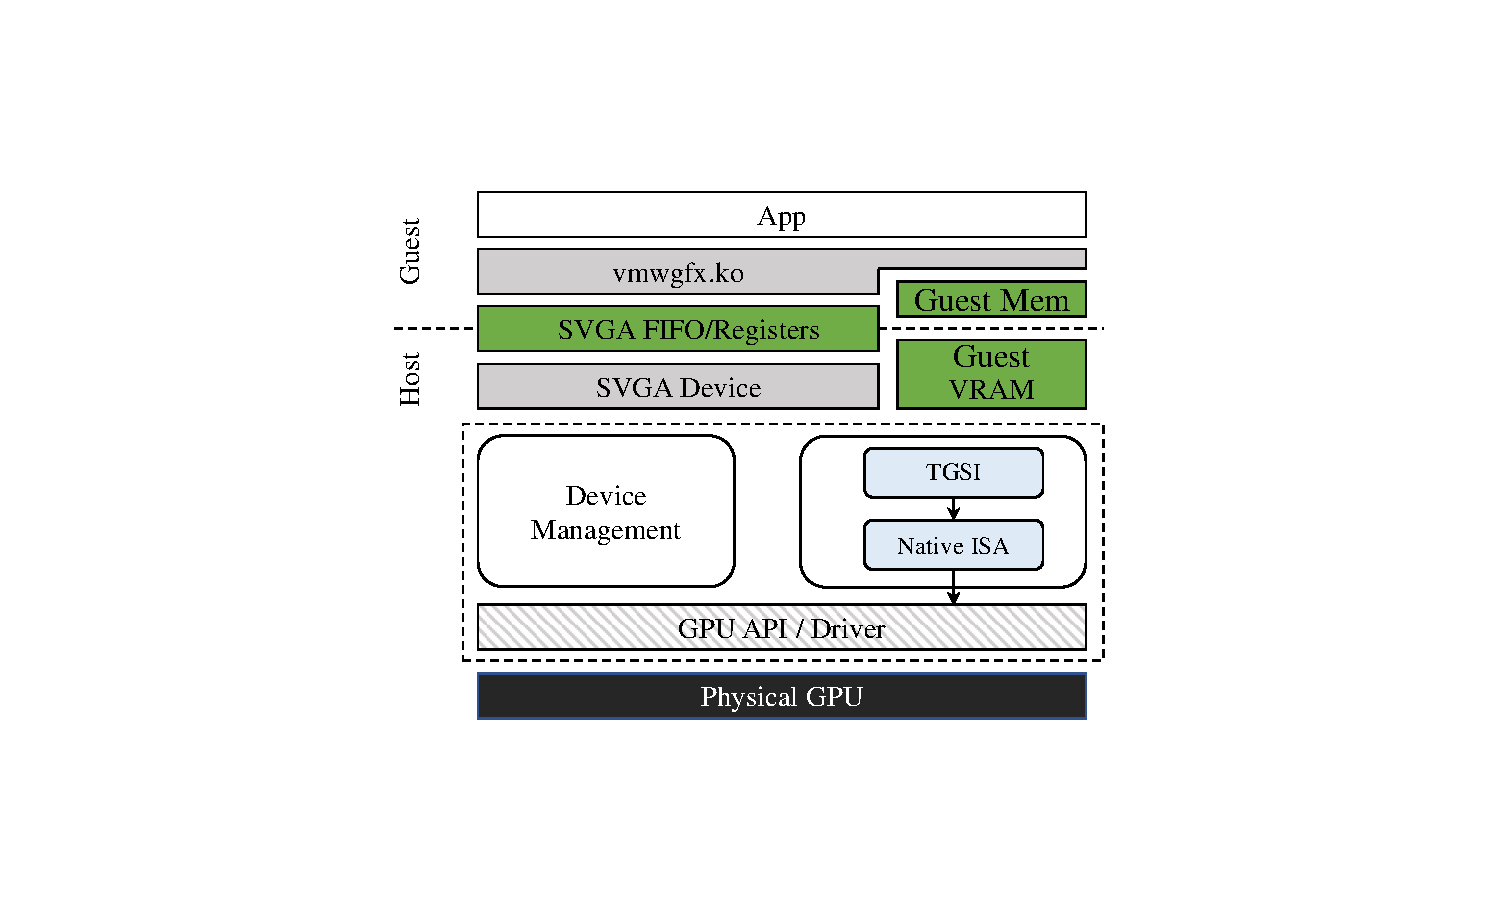
\includegraphics[width=.75\linewidth,trim={6cm 3cm 6cm 3cm},clip]{trillium/images/svga.pdf}
	\caption{{\footnotesize The design of SVGA.}}
	\label{fig_svga} \end{figure}

\subsection{SVGA}
\label{sec:svga}

SVGA~\cite{dowty2009gpu} remotes DirectX and OpenGL over an emulated (software) PCIe device.
The SVGA virtual device behaves like a physical GPU, by exporting virtual resources
in the form of registers, extents of guest memory accessible to the virtual device,
and a command queue.
I/O registers (used for mode switching, IRQs, memory allocation) are mapped
in an interposed PCIe Base Address Register (BAR) to enable synchronous emulation.
Access to GPU memory is supported through asynchronous DMA.
Figure~\ref{fig_svga} presents an overview of SVGA.

SVGA combines many aspects of full-, para-virtual and API remoting designs.
Unmodified guests can transparently use SVGA as a VGA device, making full
virtualization possible where necessary. However, access to GPU acceleration
requires para-virtualization through VMware's guest driver.
% Like a physical GPU,
SVGA processes commands from a memory mapped command queue;
% unlike a physical GPU, the command queue can be
% directly accessed by the hypervisor,
the command queue functions as a transport layer for protocols
between the guest graphics stack and the hypervisor.

SVGA uses the DirectX~\cite{directX} API as its internal protocol, thereby
realizing an API-remoting design. The transport layer and protocol are
completely under the control of the hypervisor, enabling many of the benefits
of API-remoting while ameliorating its downsides. However, using the DirectX
API as a transport protocol requires that
the driver and hypervisor translate guest interactions into DirectX
whether they are natively expressed in DirectX or not.
Coupling the transport layer with a particular version of the DirectX protocol has led to
serious complexity and compatibility \textit{challenges}: supporting each new version of the API
takes many person-years (VMware introduced support for DirectX 10 (introduced in 2006)
in 2015!).
SVGA also supports a virtual GPU ISA called TGSI~\cite{tgsi}.
% Originally developed for graphics,
TGSI maps naturally to the graphics features of the ISAs it was
originally designed to encapsulate, but has failed to keep up with
GPU ISAs that have evolved to support general purpose computation primitives.
% , TGSI has failed to evolve with it.

%SVGA's design for marshaling guest graphics stack
%calls to and from the DirectX API is essential to providing
%interactive graphics performance.
%However, the choice of a single API forces translation
%to and from other framework APIs,
%and mapping TGSI to all possible physical GPU ISAs
%creates a significant compatibility problem which over time
%has introduced staggering software complexity;
%SVGA has consequently failed to keep up with evolution of
%graphics frameworks despite monumental engineering effort.

\subsection{Mesa3D OpenCL Support}

The Mesa3D Graphics Library~\cite{mesa} is an open-source graphics
framework that implements graphics runtime libraries (e.g., OpenGL~\cite{openGLspec}, Vulkan~\cite{Vulkanspec}, Direct3D~\cite{directX}, and OpenCL~\cite{stone2010opencl})
% It is the default graphics stack
on most GNU/Linux installations.
% Mesa3D includes support for  and others.
It also includes official device drivers, written in a common framework, Gallium3D~\cite{gallium}, for Intel and AMD GPUs.
Support for NVIDIA GPUs is provided via reverse-engineered open-source Nouveau driver. Gallium3D imposes TGSI as the common
virtual ISA for compute shaders, and decomposes drivers into two
components: \textit{state trackers}, which keep track of the device
state, and \textit{pipe drivers}, which provide an interface for
controlling the GPU's graphics pipeline.
% (e.g. translate the state, shaders, and primitives into something that the hardware understands).
% Effort is underway to replace TGSI with
% SPIR-V and LLVM IR, but it wasn't mature when we undertook this project.

OpenCL support was first introduced in Mesa3D 9.0 with the release of the
Clover state tracker.
% Clover supports OpenCL~1.1 and was mainly contributed by AMD developers.
It was envisioned that Clover would leverage the LLVM~\cite{lattner2004llvm}
compiler to lower the OpenCL source to TGSI. Despite much effort by the
open-source community~\cite{old_llvm_tgsi1,old_llvm_tgsi2}, an LLVM TGSI back-end
has remained incomplete.
% Contributed by AMD developers and open-source community, Clover supports OpenCL~1.1 on most AMD GPUs.
% However, because AMD started to focus upon their ROCm compute platform~\cite{amd_rocm},
% Clover has not kept up with the fast upgrades of vendor hardware and
% software systems.
Clover currently supports an incomplete set of OpenCL~1.1 APIs on AMD GPUs and fails to operate
correctly on NVIDIA GPUs.

\subsection{GPU ISAs and IRs}

GPU front-end compilers produce code in virtual ISAs (NVIDIA PTX and LLVM IR for AMD) which are subsequently finalized using JIT compilers in the GPU driver to the native ISA (SASS and GCN).
The vISA remains stable across generations to preserve compatibility, while
the physical ISA is free to evolve. TGSI, the virtual ISA used in both the Mesa
stack and SVGA, plays a similar role---enabling interoperability
between graphics frameworks and GPUs from different vendors.
An improved virtual ISA, SPIR-V, has been proposed as a new standard~\cite{Vulkanspec} and an effort is under way to replace TGSI with SPIR-V in the Mesa3D stack.
%When standardization works, interoperability and compatibility are much easier
%to achieve.
%IRs, such as TGSI, designed by driver frameworks end up being too intertwined
%with their frameworks to keep up with the fast pace of evolution in the
%HW, or don't achieve critical mass.

LLVM has become the de-facto standard for building compilers:
both NVIDIA and AMD use it to implement their virtual ISA compilers,
as do all the compilers in the Mesa stack including the TGSI compiler we implemented.
LLVM IR is in a unique position to become a standard IR.
%The framework supports a wide array of front-end languages including CUDA and OpenCL among others, and a wide array of back-ends as well, including other IRs like SPIR-V.

%% Intermediate Representations are incredibly useful tools to hardware vendors, enabling them to simultaneously:
%% \begin{compactitem}
%% \item preserve backward compatibility without compromising innovation at the ISA. By having a publicly available ISA, that has longevity, and can be then be translated to a set of instructions that doesn't need to be preserved across generations
%% \item have the ability to reoptimize legacy code for new HW without having a dependency on the high level toolkit that generated the code in the first place
%% \item have the freedom to optimize their hardware any way they see fit without having to worry about the effect of said optimizations on the ISA
%% \item simplify their tool-chain building process by having to only modify
%% one piece (the finalizer: the piece that translates from IR to physical ISA) with each new generation of HW
%% \item leverage open source frameworks like LLVM without having to give up their secret sauce
%% \end{compactitem}
%% Given these properties, it comes as no surprise that both AMD and Nvidia have
%% both a public virtual ISA that is stable across generations i.e. IL and PTX
%% respectively, and a physical ISA that is free to evolve with each generation
%% of hardware, i.e. GCN and SASS respectively. IRs are of great interest to
%% in the realm of virtualization because an IR that is expressive enough to be
%% able to take advantage of new HW developments, while also being universally
%% accepted by all the competing parties will make a wonderful GPGPU virtualization primitive.

%% As is often the case in a space where competition is fierce, standardization
%% is hard to come by. Despite efforts by standards organizations~\cite{Vulkanspec} to convince competing parties to find a middle ground, so as to give tool
%% writers some semblance of sanity, no clear standard IR has emerged in the
%% GPGPU realm. SPIR-V~\footnote{https://www.khronos.org/spir/} is the latest
%% challenger to walk this gauntlet.

%% IRs, such as TGSI, designed by driver frameworks end up being too intertwined
%% with their frameworks to keep up with the fast pace of evolution in the
%% HW, or don't achieve critical mass.

%% Interestingly, an unlikely candidate may have emerged that is viable as a
%% virtualization primitive: LLVM IR. As a function of being the compiler
%% framework that both Nvidia and AMD use to implement their virtual ISA
%% compilers, LLVM IR is in a unique position to be the candidate IR for GPGPU
%% virtualization frameworks. The framework supports a wide array of front-end languages including CUDA and OpenCL among others, and a wide array of back-ends as well, including other IRs like SPIR-V.

% \input{framework-dims}

